% MobileDeepfake Master's Defense Presentation
% LaTeX Beamer Presentation
% Compile with: xelatex defense_slides.tex

\documentclass[aspectratio=169,12pt]{beamer}

% ============================================
% Theme and Color Configuration
% ============================================
\usetheme{Madrid}
\usecolortheme{whale}
\useinnertheme{rectangles}

% Custom colors
\definecolor{primaryblue}{RGB}{0,83,155}
\definecolor{secondaryblue}{RGB}{70,130,180}
\definecolor{alertred}{RGB}{192,0,0}
\definecolor{successgreen}{RGB}{0,128,0}
\definecolor{PolyUred}{RGB}{198,12,48}

\setbeamercolor{structure}{fg=primaryblue}
\setbeamercolor{block title}{bg=primaryblue,fg=white}
\setbeamercolor{block body}{bg=primaryblue!10}
\setbeamercolor{alerted text}{fg=alertred}

% ============================================
% PolyU Background Design (DISABLED)
% ============================================
% \setbeamertemplate{background canvas}{
%   \begin{tikzpicture}[remember picture, overlay]
%     % Top bar - PolyU Red
%     \fill[PolyUred] (current page.north west) rectangle ($(current page.north east) + (0, -0.9cm)$);
%     % Bottom bar - PolyU Red
%     \fill[PolyUred] (current page.south west) rectangle ($(current page.south east) + (0, 0.9cm)$);
%   \end{tikzpicture}
% }
%
% \setbeamertemplate{background}{
%   \begin{tikzpicture}[remember picture, overlay]
%     % Top bar - PolyU Red
%     \fill[PolyUred] (current page.north west) rectangle ($(current page.north east) + (0, -0.9cm)$);
%     % Bottom bar - PolyU Red
%     \fill[PolyUred] (current page.south west) rectangle ($(current page.south east) + (0, 0.9cm)$);
%   \end{tikzpicture}
% }

% ============================================
% Packages
% ============================================
\usepackage{graphicx}
\usepackage{booktabs}
\usepackage{tikz}
\usepackage{pgfplots}
\usepackage{amsmath,amssymb}
\usepackage{multirow}
\usepackage{array}
\usepackage{fontspec}

% Chinese Support - Comment out if not needed
\usepackage{xeCJK}
\setCJKmainfont{STHeiti}
\setCJKsansfont{STHeiti}
\setCJKmonofont{STFangsong}

% TikZ libraries
\usetikzlibrary{shapes,arrows,positioning,calc,fit,backgrounds}
\pgfplotsset{compat=1.18}

% ============================================
% Graphics Path
% ============================================
\graphicspath{{../../paper/figures/}}

% ============================================
% Document Metadata
% ============================================
\title[MobileDeepfake]{MobileDeepfake}
\subtitle{A Lightweight Cascaded Deepfake Detection System for Mobile Deployment}
\author{Wing Yam Ho}
\institute{The Hong Kong Polytechnic University}
\date{December 2025}

% Additional title page information
\newcommand{\supervisor}{Zhou Kai}
\newcommand{\department}{DSAI}
\newcommand{\program}{MScAIBDC (62037)}

% ============================================
% Custom Commands
% ============================================
\newcommand{\highlight}[1]{\textcolor{primaryblue}{\textbf{#1}}}
\newcommand{\alerttext}[1]{\textcolor{alertred}{\textbf{#1}}}
\newcommand{\successtext}[1]{\textcolor{successgreen}{\textbf{#1}}}

% Navigation symbols
\setbeamertemplate{navigation symbols}{}

% Footer
\setbeamertemplate{footline}{
  \leavevmode%
  \hbox{%
    \begin{beamercolorbox}[wd=.333333\paperwidth,ht=2.25ex,dp=1ex,center]{author in head/foot}%
      \usebeamerfont{author in head/foot}\insertshortauthor
    \end{beamercolorbox}%
    \begin{beamercolorbox}[wd=.333333\paperwidth,ht=2.25ex,dp=1ex,center]{title in head/foot}%
      \usebeamerfont{title in head/foot}\insertshorttitle
    \end{beamercolorbox}%
    \begin{beamercolorbox}[wd=.333333\paperwidth,ht=2.25ex,dp=1ex,right]{date in head/foot}%
      \usebeamerfont{date in head/foot}\insertframenumber{} / \inserttotalframenumber\hspace*{2ex}
    \end{beamercolorbox}}%
  \vskip0pt%
}

% ============================================
% Document Begin
% ============================================
\begin{document}

% ============================================
% Slide 1: Title
% ============================================
\begin{frame}
\begin{center}
\vspace*{1.5cm}
{\Huge \textbf{\inserttitle}}

\vspace{1em}
{\large \insertsubtitle}

\vspace{1em}
{\Large \insertauthor}

\vspace{0.5em}
{\normalsize \insertinstitute}

\vspace{1.5em}
{\small Supervisor: \supervisor}

\vspace{0.3em}
{\small Department: \department}

\vspace{0.3em}
{\small Program: \program}

\vfill
{\normalsize \insertdate}
\end{center}
\end{frame}

% ============================================
% Slide 2: Research Background
% ============================================
\begin{frame}{Research Background}
\begin{columns}[T]
\begin{column}{0.5\textwidth}
\textbf{Deepfake Technology Evolution}
\begin{itemize}
    \item GAN and Diffusion-based face synthesis
    \item Photorealistic quality that often fools humans
    \item Low barrier, wide accessibility
\end{itemize}

\vspace{0.5em}
\textbf{Social Risks}
\begin{itemize}
    \item Political misinformation
    \item Financial fraud via celebrity/synthetic identities
    \item Non-consensual intimate imagery
\end{itemize}
\end{column}

\begin{column}{0.5\textwidth}
\textbf{Mobile Detection Demand}
\begin{itemize}
    \item \highlight{60\%+} internet traffic from mobile
    \item Users need local content verification
    \item Privacy: sensitive data stays on-device
\end{itemize}

\vspace{1em}
\begin{block}{Key Insight}
Real-time, accurate deepfake detection on mobile devices is an urgent research direction.
\end{block}
\end{column}
\end{columns}
\end{frame}

% ============================================
% Slide 2.5: Detection Gaps and Mobile Challenges
% ============================================
\begin{frame}{Detection Gaps and Mobile Challenges}
\begin{columns}[T]
\begin{column}{0.55\textwidth}
\textbf{Benchmark vs. Real World}
\begin{itemize}
\setlength\itemsep{0.1em}
    \item Models trained on curated datasets (FF++, CelebDF)
    \item \alerttext{20--30\% AUC drop} on in-the-wild data
    \item Dataset bias and domain shift issues
\end{itemize}

\vspace{0.3em}
\textbf{Server-Centric Assumptions}
\begin{itemize}
\setlength\itemsep{0.1em}
    \item Most work evaluates on server-class GPUs
    \item Limited attention to mobile/edge devices
    \item Mobile-specific metrics rarely reported
\end{itemize}
\end{column}

\begin{column}{0.45\textwidth}
\textbf{Mobile Deployment Constraints}
\begin{center}
\begin{tabular}{lr}
\toprule
\textbf{Constraint} & \textbf{Target} \\
\midrule
Model Size & $\leq$ 100 MB \\
Latency & $<$ 200 ms \\
Energy & Battery-friendly \\
Privacy & On-device only \\
\bottomrule
\end{tabular}
\end{center}

\vspace{0.5em}
\begin{block}{Research Gap}
No existing cascade detector provides explicit FNR control with auditable cost-risk trade-offs for mobile.
\end{block}
\end{column}
\end{columns}
\end{frame}

% ============================================
% Slide 3: Problems and Challenges
% ============================================
\begin{frame}{Problems and Challenges}
\begin{center}
\renewcommand{\arraystretch}{1.0}
\footnotesize
\begin{tabular}{>{\raggedright}p{4cm} p{10cm}}
\toprule
\textbf{Challenge} & \textbf{Description} \\
\midrule
\alerttext{Lightweight vs. Accuracy} & High-precision models are computationally heavy; mobile resources are limited \\
\alerttext{Distribution Shift} & Training data differs significantly from real-world application scenarios \\
\alerttext{FNR Control} & Strict false negative control under operational compute budgets \\
\alerttext{Engineering Deployment} & Complete pipeline needed: from research model to deployable system \\
\bottomrule
\end{tabular}
\end{center}

\vspace{0.1em}
\begin{block}{\footnotesize Research Questions}
\footnotesize
\begin{itemize}
\setlength\itemsep{-0.05em}
    \item How to achieve high recall under distribution shift on resource-constrained mobile devices?
    \item Can a cascaded architecture with explicit thresholds offer interpretable cost-risk trade-offs?
    \item What minimal scripts and artifacts are needed for a reproducible, auditable end-to-end system?
    \item How to evaluate robustness (compression, noise, blur) and cross-dataset generalization for deployment?
\end{itemize}
\end{block}
\end{frame}

% ============================================
% Slide 3.5: Technical Challenges in Detail
% ============================================
\begin{frame}{Technical Challenges in Detail}
\begin{columns}[T]
\begin{column}{0.55\textwidth}
\footnotesize
\textbf{False Negative Control}
\begin{itemize}
\setlength\itemsep{0.02em}
    \item Missed fakes have \alerttext{high cost} (misinformation spread)
    \item Must maintain FNR $<$ 1\% under compute budget
    \item Requires explicit, auditable threshold tuning
\end{itemize}

\vspace{0.08em}
\textbf{Probability Calibration}
\begin{itemize}
\setlength\itemsep{0.02em}
    \item Raw model scores often miscalibrated
    \item Temperature scaling for reliable confidence
    \item Essential for threshold-based decisions
\end{itemize}

\vspace{0.08em}
\textbf{Robustness Under Perturbations}
\begin{itemize}
\setlength\itemsep{0.02em}
    \item JPEG compression, noise, blur in real media
    \item Multi-platform effects (filters, subtitles)
    \item Need systematic evaluation protocol
\end{itemize}
\end{column}

\begin{column}{0.45\textwidth}
\textbf{Trade-off Analysis}
\begin{center}
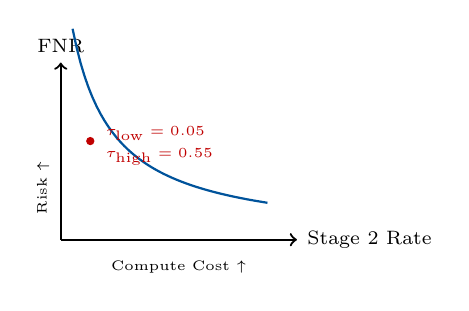
\begin{tikzpicture}[scale=0.75]
    % Axes
    \draw[->, thick] (0,0) -- (4,0) node[right, font=\scriptsize] {Stage 2 Rate};
    \draw[->, thick] (0,0) -- (0,3) node[above, font=\scriptsize] {FNR};

    % Curve
    \draw[thick, primaryblue, domain=0.2:3.5, samples=50] plot (\x, {2.5/(\x+0.5)});

    % Point
    \fill[alertred] (0.5, 1.67) circle (2pt);
    \node[right, font=\tiny, alertred] at (0.6, 1.8) {$\tau_{\text{low}}=0.05$};
    \node[right, font=\tiny, alertred] at (0.6, 1.4) {$\tau_{\text{high}}=0.55$};

    % Labels
    \node[below, font=\tiny] at (2, -0.2) {Compute Cost $\uparrow$};
    \node[left, font=\tiny, rotate=90] at (-0.3, 1.5) {Risk $\uparrow$};
\end{tikzpicture}
\end{center}

\vspace{0.3em}
\begin{block}{Core Insight}
Explicit thresholds enable \highlight{auditable} cost-risk trade-offs, unlike black-box ensemble methods.
\end{block}
\end{column}
\end{columns}
\end{frame}

% ============================================
% Slide 4: Research Objectives and Contributions
% ============================================
\begin{frame}{Research Objectives and Contributions}
\begin{columns}[T]
\begin{column}{0.75\textwidth}
\textbf{Four Major Contributions:}

\begin{enumerate}
    \item \highlight{Cost-Aware Two-Stage Cascade}
    \begin{itemize}
        \item MobileNetV4 fast filter + EfficientNetV2-B3 expert
        \item Dual-threshold mechanism for explicit FNR control
    \end{itemize}

    \item \highlight{Multi-Dataset Training \& Cross-Dataset Evaluation}
    \begin{itemize}
        \item 4 academic datasets joint training
        \item Deepfake-Eval-2024 independent OOD test
    \end{itemize}

    \item \highlight{End-to-End Reproducible Pipeline}
    \begin{itemize}
        \item 6-stage complete workflow
    \end{itemize}

    \item \highlight{Mobile Deployment Solution}
    \begin{itemize}
        \item INT8 quantization, ONNX export
        \item Android application integration
    \end{itemize}
\end{enumerate}
\end{column}

\begin{column}{0.25\textwidth}
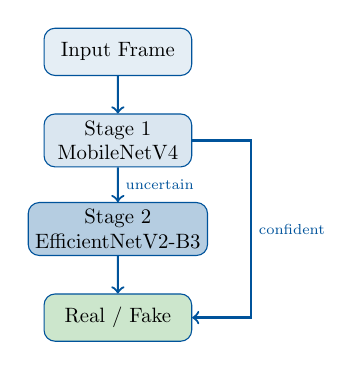
\begin{tikzpicture}[scale=0.75, transform shape,
    box/.style={rectangle, draw=primaryblue, fill=primaryblue!10,
                minimum width=2.5cm, minimum height=0.8cm, align=center, rounded corners},
    arrow/.style={->, thick, primaryblue}]

    \node[box] (input) at (0,4) {Input Frame};
    \node[box, fill=secondaryblue!20] (s1) at (0,2.5) {Stage 1\\MobileNetV4};
    \node[box, fill=secondaryblue!40] (s2) at (0,1) {Stage 2\\EfficientNetV2-B3};
    \node[box, fill=successgreen!20] (out) at (0,-0.5) {Real / Fake};

    \draw[arrow] (input) -- (s1);
    \draw[arrow] (s1) -- node[right, font=\scriptsize] {uncertain} (s2);
    \draw[arrow] (s2) -- (out);
    \draw[arrow] (s1.east) -- ++(1,0) |- node[near start, right, font=\scriptsize] {confident} (out.east);
\end{tikzpicture}
\end{column}
\end{columns}
\end{frame}

% ============================================
% Slide 4.5: Contributions – Technical Details
% ============================================
\begin{frame}{Contributions – Technical Details}
\small
\begin{columns}[T]
\begin{column}{0.5\textwidth}
\textbf{1. Cost-Aware Cascade}
\begin{itemize}
\setlength\itemsep{0.03em}
    \item Stage-1 leakage + Stage-2 escalation as \highlight{system metrics}
    \item Cost-sensitive grid search for threshold tuning
    \item Optional Stage-3 LightGBM (analysis only)
\end{itemize}

\textbf{2. Cross-Dataset Evaluation}
\begin{itemize}
\setlength\itemsep{0.03em}
    \item Quantify \alerttext{cross-dataset gaps} and failure modes
    \item Compare single-model vs cascade
    \item Calibrated vs uncalibrated thresholds
\end{itemize}
\end{column}

\begin{column}{0.5\textwidth}
\textbf{3. Scriptable Pipeline}
\begin{itemize}
\setlength\itemsep{0.03em}
    \item Data preprocessing + manifest generation
    \item Hard-example mining (HEM)
    \item Calibration + robustness sweeps
    \item Scripts reproduce all thesis tables/figures
\end{itemize}


\textbf{4. Mobile Export Template}
\begin{itemize}
\setlength\itemsep{0.03em}
    \item INT8 quantization + knowledge distillation
    \item TorchScript (primary) + ONNX export
    \item Metadata file: thresholds + temperature
    \item Reusable Android integration template
\end{itemize}
\end{column}
\end{columns}

\vspace{0.2em}
\begin{block}{\small Design Philosophy}
\small Bridge the gap between \highlight{research prototype} and \highlight{auditable mobile deployment} with explicit, reproducible controls.
\end{block}
\end{frame}

% ============================================
% Slide 5: Two-Stage Cascade Design
% ============================================
\begin{frame}{Two-Stage Cascade Design}
\begin{columns}[T]
\begin{column}{0.5\textwidth}
\textbf{Design Motivation}
\begin{itemize}
    \item Target: \highlight{$\sim$180ms} latency on mobile
    \item Balance accuracy, energy, and speed
\end{itemize}

\vspace{0.5em}
\textbf{Stage 1: MobileNetV4}
\begin{itemize}
    \item Fast, lightweight filter
    \item AUC = \highlight{0.9936}
    \item Size: 37.3 MB
\end{itemize}

\vspace{0.5em}
\textbf{Stage 2: EfficientNetV2-B3}
\begin{itemize}
    \item Processes only uncertain samples
    \item AUC = 0.9633
    \item Size: 49.6 MB
\end{itemize}
\end{column}

\begin{column}{0.5\textwidth}


\vspace{1em}
\begin{block}{Cascade Effect}
\begin{itemize}
    \item FNR $\approx$ \successtext{0.6\%}
    \item Stage 2 escalation: only \successtext{$\sim$1.2\%}
    \item Most samples resolved at Stage 1
\end{itemize}
\end{block}
\end{column}
\end{columns}
\end{frame}

% ============================================
% Slide 5.5: Cascade Efficiency & Operating Points
% ============================================
\begin{frame}{Cascade Efficiency \& Operating Points}
\small
\begin{columns}[T]
\begin{column}{0.55\textwidth}
\textbf{Compute Cost Comparison}
\begin{center}
\scriptsize
\begin{tabular}{lrrr}
\toprule
\textbf{Configuration} & \textbf{GFLOPs} & \textbf{FNR} & \textbf{Stage2} \\
\midrule
Stage 1 only & 0.54 & 3.12\% & -- \\
Stage 2 only & 2.87 & 9.43\% & 100\% \\
\midrule
\textbf{Cascade} & \highlight{0.59} & \successtext{0.60\%} & 1.16\% \\
\bottomrule
\end{tabular}
\end{center}

\vspace{0.15em}
\textbf{Quantization Impact}
\begin{itemize}
\setlength\itemsep{0.03em}
    \item Stage 1: 37.3 MB $\rightarrow$ \highlight{10.1 MB} (INT8)
    \item Stage 2: 49.6 MB $\rightarrow$ \highlight{13.4 MB} (INT8)
    \item AUC loss: $<$ 0.01 per stage
\end{itemize}
\end{column}

\begin{column}{0.45\textwidth}
\textbf{Deployment Scenarios}
\begin{center}
\scriptsize
\begin{tabular}{lcc}
\toprule
\textbf{Scenario} & $\tau_{\text{low}}/\tau_{\text{high}}$ & \textbf{FNR} \\
\midrule
Safety-first & 0.05 / 0.55 & 0.60\% \\
Balanced & 0.10 / 0.50 & 1.2\% \\
Speed-first & 0.15 / 0.45 & 2.0\% \\
\bottomrule
\end{tabular}
\end{center}

\vspace{0.1em}
\textbf{Calibration Effect}
\begin{itemize}
\setlength\itemsep{0.03em}
    \item Temperature scaling: T $\approx$ 1.34
    \item ECE reduced by \highlight{79\%}
    \item Enables reliable threshold decisions
\end{itemize}
\end{column}
\end{columns}

\vspace{0.05em}
\begin{block}{\footnotesize Key Insight}
\footnotesize Cascade: \successtext{5$\times$ lower FNR} than Stage 1 alone \quad with only \highlight{9\%} compute overhead.
\end{block}
\end{frame}

% ============================================
% Slide 6: Cascade Decision Logic
% ============================================
\begin{frame}{Cascade Decision Logic}
\begin{columns}[T]
\begin{column}{0.55\textwidth}
\textbf{Dual-Threshold Mechanism}

Stage 1 output: $p_1(x) = P(\text{fake} \mid x)$

\begin{itemize}
    \item Low threshold: $\tau_{\text{low}} = 0.05$
    \item High threshold: $\tau_{\text{high}} = 0.55$
\end{itemize}

\textbf{Decision Rules:}
\[
\hat{y}(x) = \begin{cases}
\text{real}, & \text{if } p_1(x) < \tau_{\text{low}} \\
\text{fake}, & \text{if } p_1(x) > \tau_{\text{high}} \\
\text{Stage2}(x), & \text{otherwise}
\end{cases}
\]

\textbf{Stage 2 Decision:}
\begin{itemize}
    \item $p_2(x) > 0.5 \Rightarrow$ Fake
    \item $p_2(x) \leq 0.5 \Rightarrow$ Real
\end{itemize}
\end{column}

\begin{column}{0.45\textwidth}
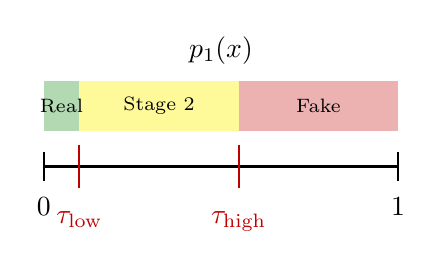
\begin{tikzpicture}[scale=0.9]
    % Confidence bar
    \draw[thick] (0,0) -- (5,0);
    \draw[thick] (0,-0.2) -- (0,0.2);
    \draw[thick] (5,-0.2) -- (5,0.2);

    % Threshold lines
    \draw[thick, alertred] (0.5,-0.3) -- (0.5,0.3);
    \draw[thick, alertred] (2.75,-0.3) -- (2.75,0.3);

    % Labels
    \node[below] at (0,-0.3) {0};
    \node[below] at (5,-0.3) {1};
    \node[below, alertred] at (0.5,-0.5) {$\tau_{\text{low}}$};
    \node[below, alertred] at (2.75,-0.5) {$\tau_{\text{high}}$};

    % Regions
    \fill[successgreen!30] (0,0.5) rectangle (0.5,1.2);
    \fill[yellow!40] (0.5,0.5) rectangle (2.75,1.2);
    \fill[alertred!30] (2.75,0.5) rectangle (5,1.2);

    \node[font=\scriptsize] at (0.25,0.85) {Real};
    \node[font=\scriptsize] at (1.625,0.85) {Stage 2};
    \node[font=\scriptsize] at (3.875,0.85) {Fake};

    % p1(x) label
    \node[above] at (2.5,1.3) {$p_1(x)$};
\end{tikzpicture}

\vspace{1em}
\begin{block}{Performance}
\begin{itemize}
    \item FNR $\approx$ 0.6\%
    \item Escalation rate $\approx$ 1.2\%
\end{itemize}
\end{block}
\end{column}
\end{columns}
\end{frame}

% ============================================
% Slide 7: Six-Stage Pipeline
% ============================================
\begin{frame}{Six-Stage Pipeline}
\begin{center}
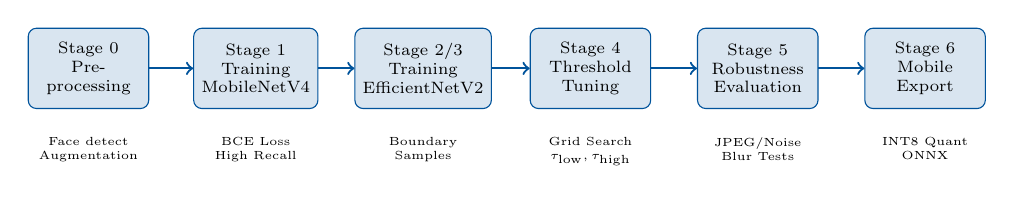
\begin{tikzpicture}[scale=0.85, transform shape,
    stage/.style={rectangle, draw=primaryblue, fill=primaryblue!15,
                  minimum width=1.8cm, minimum height=1.2cm, align=center,
                  rounded corners=3pt, font=\scriptsize},
    arrow/.style={->, thick, primaryblue}]

% Stages
\node[stage] (s1) at (0,0) {Stage 0\\Pre-\\processing};
\node[stage] (s2) at (2.5,0) {Stage 1\\Training\\MobileNetV4};
\node[stage] (s3) at (5,0) {Stage 2/3\\Training\\EfficientNetV2};
\node[stage] (s4) at (7.5,0) {Stage 4\\Threshold\\Tuning};
\node[stage] (s5) at (10,0) {Stage 5\\Robustness\\Evaluation};
\node[stage] (s6) at (12.5,0) {Stage 6\\Mobile\\Export};

% Arrows
\draw[arrow] (s1) -- (s2);
\draw[arrow] (s2) -- (s3);
\draw[arrow] (s3) -- (s4);
\draw[arrow] (s4) -- (s5);
\draw[arrow] (s5) -- (s6);

% Key points below
\node[below=0.3cm of s1, font=\tiny, align=center] {Face detect\\Augmentation};
\node[below=0.3cm of s2, font=\tiny, align=center] {BCE Loss\\High Recall};
\node[below=0.3cm of s3, font=\tiny, align=center] {Boundary\\Samples};
\node[below=0.3cm of s4, font=\tiny, align=center] {Grid Search\\$\tau_{\text{low}}, \tau_{\text{high}}$};
\node[below=0.3cm of s5, font=\tiny, align=center] {JPEG/Noise\\Blur Tests};
\node[below=0.3cm of s6, font=\tiny, align=center] {INT8 Quant\\ONNX};
\end{tikzpicture}
\end{center}

\begin{center}
\begin{tabular}{clp{10cm}}
\toprule
\textbf{Stage} & \textbf{Name} & \textbf{Key Techniques} \\
\midrule
0 & Data \& Preprocess & Multi-backend face detection, 256$\times$256 crops, manifests \\
1 & Stage1 Training & MobileNetV4, BCE loss, temperature calibration \\
2 & Stage2 Training & EfficientNetV2-B3, focal loss, strong augmentation \\
3 & Meta-Model (opt.) & LightGBM on embeddings (analysis only, not deployed) \\
4 & Threshold Tuning & Grid search for $\tau_{\text{low}}/\tau_{\text{high}}$, FNR constraint \\
5 & Robustness & JPEG, noise, blur, brightness, gamma sweeps \\
6 & Mobile Export & TorchScript INT8 + FP32 ONNX, \highlight{180ms / 92.8\%} \\
\bottomrule
\end{tabular}
\end{center}
\end{frame}

% ============================================
% Slide 7.5: Mobile Deployment Details
% ============================================
\begin{frame}{Mobile Deployment Details}
\begin{columns}[T]
\begin{column}{0.5\textwidth}
\textbf{Export Artifacts}
\begin{center}
\scriptsize
\begin{tabular}{lrr}
\toprule
\textbf{Format} & \textbf{Stage 1} & \textbf{Stage 2} \\
\midrule
FP32 TorchScript & 37.3 MB & 49.6 MB \\
INT8 TorchScript & 10.1 MB & 13.4 MB \\
FP32 ONNX & 37.5 MB & 52 MB \\
\bottomrule
\end{tabular}
\end{center}

\vspace{0.3em}
\textbf{On-Device Pipeline}
\begin{itemize}
\setlength\itemsep{0.1em}
    \item FaceDetector API $\rightarrow$ 256$\times$256 crop
    \item ImageNet normalization
    \item Stage 1 $\rightarrow$ cascade routing $\rightarrow$ Stage 2
    \item Temperature scaling on logits
\end{itemize}
\end{column}

\begin{column}{0.5\textwidth}
\textbf{On-Device Metrics (Xiaomi 13)}
\begin{center}
\scriptsize
\begin{tabular}{lr}
\toprule
\textbf{Metric} & \textbf{Value} \\
\midrule
Accuracy & \highlight{92.8\%} \\
FNR & 2.5\% \\
FPR & 12.5\% \\
Stage-2 Rate & 7.2\% \\
\midrule
Preprocessing & 3.4 ms \\
Inference & 176 ms \\
\textbf{Total Latency} & \highlight{$\sim$180 ms} \\
\bottomrule
\end{tabular}
\end{center}

\vspace{0.3em}
\textbf{Runtime Stack}
\begin{itemize}
\setlength\itemsep{0.1em}
    \item ONNX Runtime Android 1.19.0
    \item CPUExecutionProvider (ARM NEON)
    \item NNAPI/GPU delegates: future work
\end{itemize}
\end{column}
\end{columns}

\vspace{0.3em}
\begin{block}{Deployment Note}
Android bundle uses \highlight{FP32 ONNX} models; INT8 TorchScript available for size-constrained scenarios with minimal AUC loss.
\end{block}
\end{frame}

% ============================================
% Slide 8: Mobile Architecture
% ============================================
\begin{frame}{Mobile Architecture}
\begin{columns}[T]
\begin{column}{0.65\textwidth}
\textbf{Model Compression}
\begin{itemize}
\setlength\itemsep{0.1em}
    \item FP32 TorchScript: 37.3MB / 49.6MB
    \item INT8 TorchScript: 10.1MB / 13.4MB
    \item FP32 ONNX (Android): $\sim$37.5MB / $\sim$52MB
\end{itemize}

\vspace{-0.3em}
\textbf{Inference Framework}
\begin{itemize}
\setlength\itemsep{0.1em}
    \item PyTorch $\rightarrow$ ONNX export
    \item ONNX Runtime Android 1.19.0 (CPU)
    \item NNAPI/GPU delegates: future work
\end{itemize}

\vspace{-0.3em}
\textbf{Key Metrics}
\begin{itemize}
\setlength\itemsep{0.1em}
    \item Latency: \highlight{$\sim$180ms}
    \item Accuracy: \highlight{92.8\%}
    \item Device: Xiaomi 13 (Snapdragon 8 Gen 2)
\end{itemize}
\end{column}

\begin{column}{0.35\textwidth}
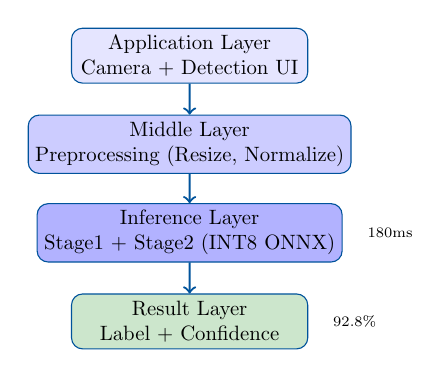
\begin{tikzpicture}[scale=0.75, transform shape,
    layer/.style={rectangle, draw=primaryblue, minimum width=4cm,
                  minimum height=0.9cm, align=center, rounded corners},
    arrow/.style={->, thick, primaryblue}]

\node[layer, fill=blue!10] (app) at (0,3.5) {Application Layer\\Camera + Detection UI};
\node[layer, fill=blue!20] (mid) at (0,2) {Middle Layer\\Preprocessing (Resize, Normalize)};
\node[layer, fill=blue!30] (inf) at (0,0.5) {Inference Layer\\Stage1 + Stage2 (INT8 ONNX)};
\node[layer, fill=successgreen!20] (out) at (0,-1) {Result Layer\\Label + Confidence};

\draw[arrow] (app) -- (mid);
\draw[arrow] (mid) -- (inf);
\draw[arrow] (inf) -- (out);

% Side annotations
\node[right=0.3cm of inf, font=\scriptsize] {180ms};
\node[right=0.3cm of out, font=\scriptsize] {92.8\%};
\end{tikzpicture}
\end{column}
\end{columns}
\end{frame}

% ============================================
% Slide 9: Dataset Introduction
% ============================================
\begin{frame}{Dataset Introduction}
\begin{columns}[T]
\begin{column}{0.55\textwidth}
\textbf{Training: 2.66M + OOD: 0.85M face crops}

\begin{center}
\scriptsize
\begin{tabular}{lrrr}
\toprule
\textbf{Dataset} & \textbf{Train} & \textbf{Val} & \textbf{Test} \\
\midrule
CelebDF-v2 & 83,599 & 17,478 & 18,037 \\
FaceForensics++ & 223,653 & 50,945 & 47,430 \\
DFDC & 721,946 & 154,919 & 154,511 \\
DeeperForensics & 844,396 & 165,854 & 172,894 \\
\midrule
\textbf{Total} & \textbf{1,873,594} & \textbf{389,196} & \textbf{392,872} \\
\bottomrule
\end{tabular}
\end{center}

\textbf{Dataset Characteristics}
\begin{itemize}
    \item CelebDF-v2: High-quality celebrity swaps
    \item FF++: Multiple manipulation methods
    \item DFDC: Facebook large-scale diverse
    \item DeeperForensics: Real-world perturbations
\end{itemize}
\end{column}

\begin{column}{0.45\textwidth}
\begin{block}{OOD Evaluation: Deepfake-Eval-2024}
\begin{itemize}
    \item Val: 451,917 / Test: 402,413
    \item \highlight{88 websites}, \highlight{52 languages}
    \item 2024 real media environment
    \item Used only for evaluation; no training
\end{itemize}
\end{block}

\textbf{Design Goal:}
\begin{itemize}
    \item Cover diverse forgery methods
    \item Various shooting conditions
    \item Evaluate generalization capability
\end{itemize}
\end{column}
\end{columns}
\end{frame}

% ============================================
% Slide 9.5: Dataset Preprocessing & Splits
% ============================================
\begin{frame}{Dataset Preprocessing \& Splits}
\begin{columns}[T]
\begin{column}{0.5\textwidth}
\textbf{Unified Preprocessing}
\begin{itemize}
\setlength\itemsep{0.08em}
    \item 256$\times$256 PNG face crops
    \item Max 50 faces per video
    \item Frame interval: 10
    \item Multi-backend face detection
\end{itemize}

\textbf{Split Protocol}
\begin{itemize}
\setlength\itemsep{0.08em}
    \item Fixed ratios: 70\% / 15\% / 15\%
    \item Official test subsets preserved (FF++)
    \item Deterministic hash-based splitting
\end{itemize}

\textbf{Balanced Manifests}
\begin{itemize}
\setlength\itemsep{0.08em}
    \item $\approx$ Equal real/fake per dataset
    \item Prevents dataset dominance in training
    \item Per-split balance maintained
\end{itemize}
\end{column}

\begin{column}{0.5\textwidth}
\textbf{Class Distribution}
\begin{center}
\scriptsize
\begin{tabular}{lrrr}
\toprule
\textbf{Dataset} & \textbf{Real} & \textbf{Fake} & \textbf{Ratio} \\
\midrule
CelebDF-v2 & 59K & 60K & 0.98 \\
FF++ & 161K & 161K & 1.00 \\
DFDC & 516K & 515K & 1.00 \\
DeeperForensics & 591K & 592K & 1.00 \\
\midrule
Eval-2024 & 366K & 488K & 0.75 \\
\bottomrule
\end{tabular}
\end{center}

\textbf{Evaluation Regimes}
\begin{enumerate}
\setlength\itemsep{0.08em}
    \item Combined validation (all 4 datasets)
    \item Per-dataset validation
    \item OOD evaluation (Deepfake-Eval-2024)
    \item balanced manifests by class and datasetfor fair multi-source learning.
\end{enumerate}
\end{column}
\end{columns}
\end{frame}

% ============================================
% Slide 10: Cross-Dataset Evaluation Protocol
% ============================================
\begin{frame}{Cross-Dataset Evaluation Protocol}
\begin{columns}[T]
\begin{column}{0.5\textwidth}
\small
\textbf{Training \& Validation}
\begin{itemize}
\setlength\itemsep{-0.05em}
    \item Only on 4 public academic datasets
    \item Reproducible splits (official test where available)
    \item Balanced manifests across all 4 datasets
\end{itemize}

\textbf{Cross-Dataset Evaluation}
\begin{itemize}
\setlength\itemsep{0.05em}
    \item \alerttext{No fine-tuning} on Deepfake-Eval-2024
    \item Direct application of trained model
    \item Simulates real deployment scenario
\end{itemize}

\vspace{0.05em}
\begin{center}
\tiny
\begin{tabular}{ll}
\toprule
\textbf{Scenario} & \textbf{Metrics} \\
\midrule
In-domain & AUC, Cascade FNR, Escalation \\
OOD & F1, FNR, Stage2 Escalation \\
\bottomrule
\end{tabular}
\end{center}

{\tiny \textit{Full tables: Acc, Precision, Recall, FPR}}
\end{column}

\begin{column}{0.5\textwidth}
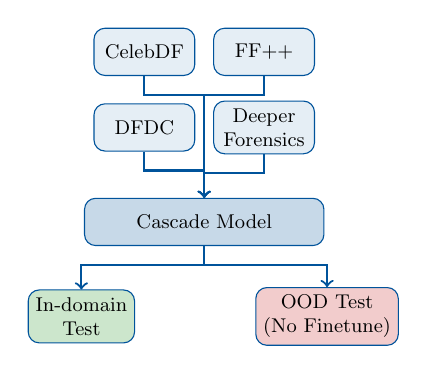
\begin{tikzpicture}[scale=0.8, transform shape,
    box/.style={rectangle, draw=primaryblue, fill=primaryblue!10,
                minimum width=1.6cm, minimum height=0.75cm, align=center,
                rounded corners, font=\small},
    arrow/.style={->, thick, primaryblue}]

% Training datasets
\node[box] (c1) at (0,3) {CelebDF};
\node[box] (c2) at (1.9,3) {FF++};
\node[box] (c3) at (0,1.8) {DFDC};
\node[box] (c4) at (1.9,1.8) {Deeper\\Forensics};

% Model
\node[box, fill=secondaryblue!30, minimum width=3.8cm] (model) at (0.95,0.3) {Cascade Model};

% Tests
\node[box, fill=successgreen!20] (in) at (-1,-1.2) {In-domain\\Test};
\node[box, fill=alertred!20] (ood) at (2.9,-1.2) {OOD Test\\(No Finetune)};

% Arrows
\draw[arrow] (c1.south) -- ++(0,-0.3) -| (model.north);
\draw[arrow] (c2.south) -- ++(0,-0.3) -| (model.north);
\draw[arrow] (c3.south) -- ++(0,-0.3) -| (model.north);
\draw[arrow] (c4.south) -- ++(0,-0.3) -| (model.north);
\draw[arrow] (model.south) -- ++(0,-0.3) -| (in.north);
\draw[arrow] (model.south) -- ++(0,-0.3) -| (ood.north);
\end{tikzpicture}

\vspace{0.3em}
\begin{block}{Goal}
Train on public data $\rightarrow$ Deploy to real internet
\end{block}
\end{column}
\end{columns}
\end{frame}

% ============================================
% Slide 11: In-domain Results
% ============================================
\begin{frame}{In-domain Results}
\begin{columns}[T]
\begin{column}{0.5\textwidth}
\textbf{Individual Stage Performance}
\begin{itemize}
    \item Stage 1 AUC: \highlight{0.9936} (F1: 0.9561)
    \item Stage 2 AUC: 0.9633 (F1: 0.8930)
\end{itemize}

\vspace{0.5em}
\textbf{Cascade Performance (Safety-first)}
\begin{itemize}
    \item Cascade AUC: \highlight{0.9941}, F1: 0.9654
    \item Final FNR: \successtext{0.60\%}
    \item Stage 2 Escalation: \successtext{1.16\%}
\end{itemize}

\vspace{0.5em}
\begin{block}{Conclusion}
On combined validation, cascade achieves high detection with significant compute savings.
\end{block}
\end{column}

\begin{column}{0.5\textwidth}
\begin{figure}
    \centering
    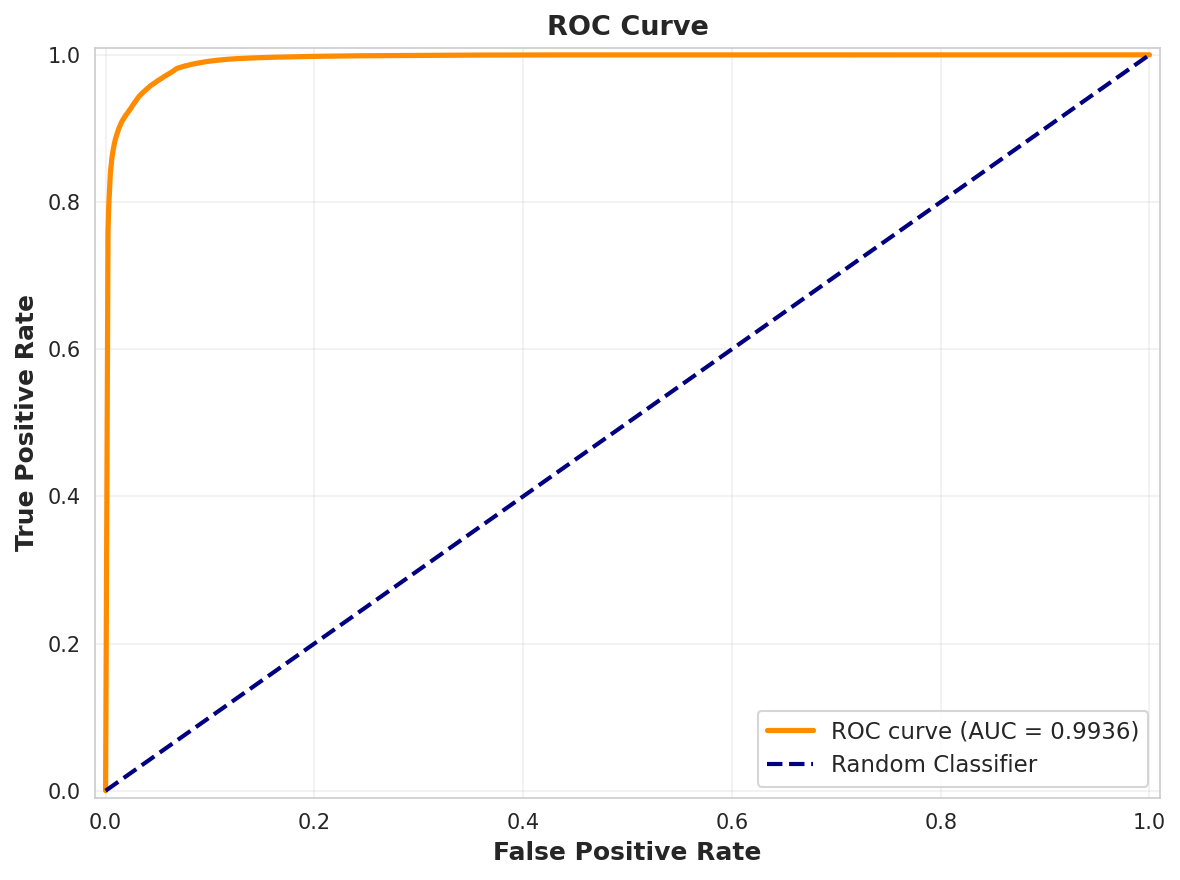
\includegraphics[width=0.9\textwidth]{outputs_stage1_run_20251023_034316_01_roc_curve.png}
    \caption*{Stage 1 ROC Curve (AUC=0.9936)}
\end{figure}
\end{column}
\end{columns}
\end{frame}

% ============================================
% Slide 11.5: Stage-wise Ablation Analysis
% ============================================
\begin{frame}{Stage-wise Ablation Analysis}
\footnotesize
\begin{columns}[T]
\begin{column}{0.5\textwidth}
\textbf{Why Cascade?}
\begin{itemize}
\setlength\itemsep{0.02em}
    \item Stage 1: Fast but higher FNR
    \item Stage 2: Lower FNR but 5$\times$ slower
    \item Cascade: Best of both worlds
\end{itemize}

\vspace{0.1em}
\textbf{Stage-wise Comparison}
\begin{center}
\tiny
\begin{tabular}{lrrrr}
\toprule
\textbf{Config} & \textbf{AUC} & \textbf{F1} & \textbf{FNR} & \textbf{GFLOPs} \\
\midrule
S1 only & 0.9936 & 0.9561 & 3.12\% & 0.54 \\
S2 only & 0.9633 & 0.8930 & 9.43\% & 2.87 \\
\midrule
\textbf{Cascade} & \textbf{0.9941} & \textbf{0.9654} & \successtext{0.60\%} & \highlight{0.59} \\
\bottomrule
\end{tabular}
\end{center}

\end{column}

\begin{column}{0.5\textwidth}
\textbf{FNR Reduction}
\begin{center}
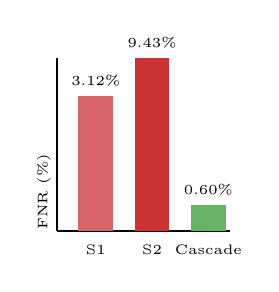
\begin{tikzpicture}[scale=0.55]
    % Bar chart
    \draw[thick] (0,0) -- (0,4);
    \draw[thick] (0,0) -- (4,0);

    % Bars
    \fill[alertred!60] (0.5,0) rectangle (1.3,3.12);
    \fill[alertred!80] (1.8,0) rectangle (2.6,4);
    \fill[successgreen!60] (3.1,0) rectangle (3.9,0.6);

    % Labels
    \node[below, font=\tiny] at (0.9,-0.1) {S1};
    \node[below, font=\tiny] at (2.2,-0.1) {S2};
    \node[below, font=\tiny] at (3.5,-0.1) {Cascade};

    % Values
    \node[above, font=\tiny] at (0.9,3.12) {3.12\%};
    \node[above, font=\tiny] at (2.2,4) {9.43\%};
    \node[above, font=\tiny] at (3.5,0.6) {0.60\%};

    % Y-axis label
    \node[left, font=\tiny, rotate=90] at (-0.3,2) {FNR (\%)};
\end{tikzpicture}
\end{center}

\vspace{-0.2em}
\textbf{Compute Efficiency}
\begin{itemize}
\setlength\itemsep{0.02em}
    \item S1: 0.54 GFLOPs
    \item S2: 2.87 GFLOPs
    \item Cascade: 0.59 GFLOPs
    \item Overhead: 9\% only
\end{itemize}
\end{column}
\end{columns}

\vspace{0.05em}
\begin{block}{\tiny Key Insight}
Cascade: \successtext{5$\times$ lower FNR} than Stage 1 \quad with only \highlight{9\%} overhead.
\end{block}
\end{frame}

% ============================================
% Slide 12: Cascade Efficiency Analysis
% ============================================
\begin{frame}{Cascade Efficiency Analysis}
\footnotesize
\begin{columns}[T]
\begin{column}{0.56\textwidth}
\textbf{Design Philosophy}
\begin{itemize}
\setlength\itemsep{0.03em}
    \item Stage 1: Lightweight, high-throughput
    \item Principle: ``Better catch more than miss''
    \item Stage 2: Fine-grained for difficult samples
\end{itemize}

\vspace{0.08em}
\textbf{Runtime Statistics}
\begin{itemize}
\setlength\itemsep{0.03em}
    \item Escalation: $\sim$1.2\%
    \item $\Rightarrow$ \highlight{98.8\%} Stage 1 only
    \item FNR: $\sim$0.6\%
\end{itemize}

\vspace{0.08em}
\textbf{Mobile/Edge Impact}
\begin{itemize}
\setlength\itemsep{0.03em}
    \item Most: fast local detection
    \item Few: optional cloud refinement
\end{itemize}
\end{column}

\begin{column}{0.44\textwidth}
\begin{figure}
    \centering
    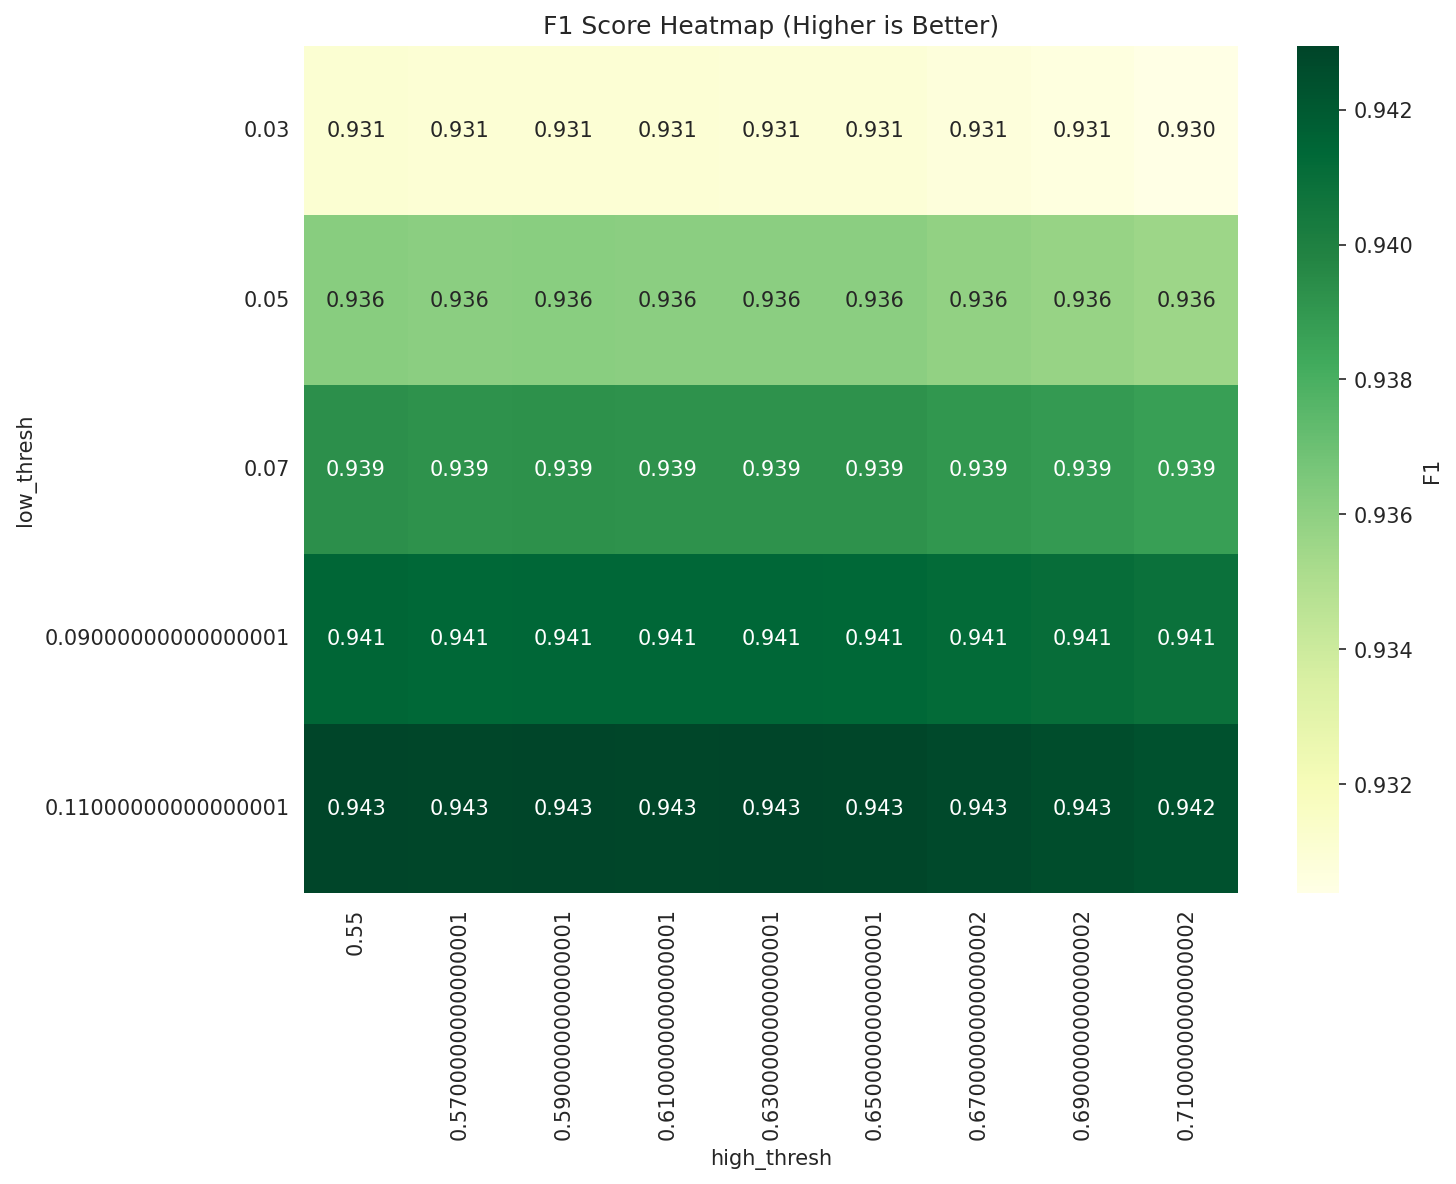
\includegraphics[width=\textwidth]{outputs_stage4_run_20251031_075851_heatmap_f1.png}
    \caption*{\tiny F1 Score Heatmap}
\end{figure}
\end{column}
\end{columns}
\end{frame}

% ============================================
% Slide 13: Mobile Performance
% ============================================
\begin{frame}{Mobile Performance}
\begin{columns}[T]
\begin{column}{0.55\textwidth}
\textbf{Test Environment}
\begin{itemize}
    \item Device: Xiaomi 13
    \item Chip: Snapdragon 8 Gen 2
\end{itemize}

\vspace{0.5em}
\begin{center}
\begin{tabular}{lr}
\toprule
\textbf{Metric} & \textbf{Value} \\
\midrule
Face-level Accuracy & \highlight{92.8\%} \\
Average Latency & \highlight{$\sim$180ms} \\
\bottomrule
\end{tabular}
\end{center}

\vspace{0.5em}
\textbf{Application Scenarios}
\begin{itemize}
    \item 25-30fps video: near real-time sampling
    \item On-device inference, no upload needed
    \item Privacy-preserving design
\end{itemize}
\end{column}

\begin{column}{0.45\textwidth}
\begin{block}{Deployment Feasibility}
Model achieves practical real-time performance on mainstream flagship smartphones.
\end{block}

\vspace{1em}
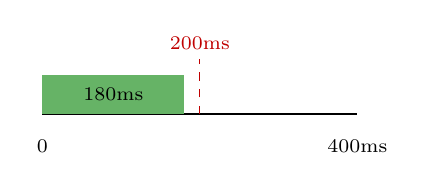
\begin{tikzpicture}
    % Latency bar
    \draw[thick] (0,0) -- (4,0);
    \fill[successgreen!60] (0,0) rectangle (1.8,0.5);
    \node at (0.9,0.25) {\scriptsize 180ms};

    % Reference line
    \draw[dashed, alertred] (2,0) -- (2,0.7);
    \node[alertred, font=\scriptsize] at (2,0.9) {200ms};

    \node[below] at (0,-0.2) {\scriptsize 0};
    \node[below] at (4,-0.2) {\scriptsize 400ms};
\end{tikzpicture}
\end{column}
\end{columns}
\end{frame}

% ============================================
% Slide 14: Cross-Dataset Challenge
% ============================================
\begin{frame}{Cross-Dataset Challenge}
\begin{columns}[T]
\begin{column}{0.55\textwidth}
\textbf{Performance Drop on Deepfake-Eval-2024}

\begin{center}
\begin{tabular}{lcc}
\toprule
\textbf{Metric} & \textbf{In-domain} & \textbf{OOD} \\
\midrule
F1 & $>$0.95 & \alerttext{$<$0.30} \\
FNR & $\sim$0.6\% & \alerttext{73-79\%} \\
FPR & $\sim$3\% & \alerttext{25-27\%} \\
Stage2 Rate & $\sim$1.2\% & \alerttext{$\sim$51\%} \\
\bottomrule
\end{tabular}
\end{center}

\textbf{Root Causes}
\begin{itemize}
    \item Training data $\neq$ 2024 internet distribution
    \item New forgery methods not in training set
    \item Domain shift from social-media processing pipelines
\end{itemize}
\end{column}

\begin{column}{0.45\textwidth}
\begin{alertblock}{Problem Revealed}
Models trained only on traditional public datasets cannot directly generalize to latest real-world scenarios.
\end{alertblock}

\vspace{0.5em}
\begin{block}{Valuable Negative Finding}
This result provides an important empirical baseline for future research on cross-domain robustness.
\end{block}
\end{column}
\end{columns}
\end{frame}

% ============================================
% Slide 14.5: OOD Analysis Deep Dive
% ============================================
\begin{frame}{OOD Analysis Deep Dive}
\begin{columns}[T]
\begin{column}{0.55\textwidth}
\textbf{Deepfake-Eval-2024 Results (Calibrated)}
\begin{center}
\scriptsize
\begin{tabular}{lrr}
\toprule
\textbf{Metric} & \textbf{Val} & \textbf{Test} \\
\midrule
F1 & 0.2996 & 0.2796 \\
Accuracy & 58.0\% & 50.0\% \\
FNR & \alerttext{72.9\%} & \alerttext{79.0\%} \\
FPR & 26.7\% & 25.1\% \\
Stage2 Rate & 51.1\% & 52.3\% \\
\bottomrule
\end{tabular}
\end{center}

\vspace{0.3em}
\textbf{Stage2-Only Baseline (Max Compute)}
\begin{center}
\scriptsize
\begin{tabular}{lrr}
\toprule
\textbf{Metric} & \textbf{Val} & \textbf{Test} \\
\midrule
F1 & 0.4460 & 0.5962 \\
FNR & 18.2\% & 14.6\% \\
FPR & \alerttext{91.6\%} & \alerttext{87.1\%} \\
Stage2 Rate & 97.5\% & 98.9\% \\
\bottomrule
\end{tabular}
\end{center}
\end{column}

\begin{column}{0.45\textwidth}
\begin{alertblock}{Key Finding}
Even with 100\% Stage 2 usage, FPR exceeds 87\% -- the problem is \alerttext{not just compute} but \highlight{domain coverage}.
\end{alertblock}

\vspace{0.3em}
\textbf{Implications}
\begin{itemize}
\setlength\itemsep{0.1em}
    \item Cascade efficiency irrelevant if base models fail
    \item Need domain adaptation / continual learning
    \item Current training data insufficient for 2024 web
\end{itemize}

\vspace{0.3em}
\begin{block}{Future Direction}
Domain generalization and periodic retraining are essential for real-world deployment.
\end{block}
\end{column}
\end{columns}
\end{frame}

% ============================================
% Slide 15: Robustness and Error Analysis
% ============================================
\begin{frame}{Robustness and Error Analysis}
\begin{columns}[T]
\begin{column}{0.55\textwidth}
\textbf{Image Perturbation Experiments}

\begin{center}
\scriptsize
\begin{tabular}{lp{5cm}}
\toprule
\textbf{Perturbation} & \textbf{Observation} \\
\midrule
JPEG Compression & Moderate compression sometimes improves F1 \\
Gaussian Noise & Moderate noise: unstable performance \\
Motion Blur & \alerttext{Near-total failure} (FNR $\sim$96-100\%) \\
\bottomrule
\end{tabular}
\end{center}

{\scriptsize \textit{Note: Robustness results are sample-limited and treated as preliminary hypotheses.}}

\textbf{Typical Failure Cases}
\begin{itemize}
    \item High-quality fakes: human-indistinguishable
    \item Extreme compression: texture destroyed
    \item Occlusion/non-standard: masks, filters, backlighting
\end{itemize}
\end{column}

\begin{column}{0.45\textwidth}
\begin{figure}
    \centering
    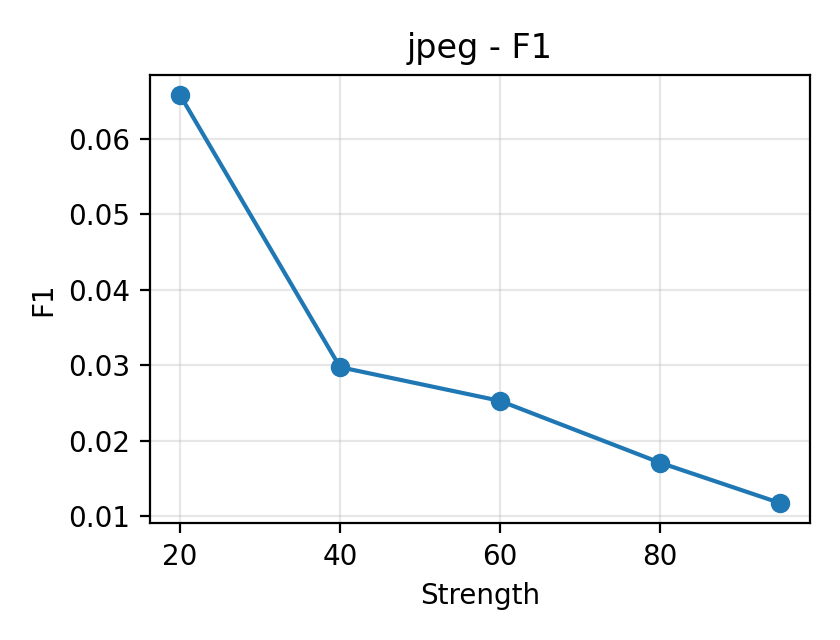
\includegraphics[width=0.9\textwidth]{outputs_stage5_robustness_jpeg_f1.png}
    \caption*{JPEG Quality vs F1}
\end{figure}

\begin{figure}
    \centering
    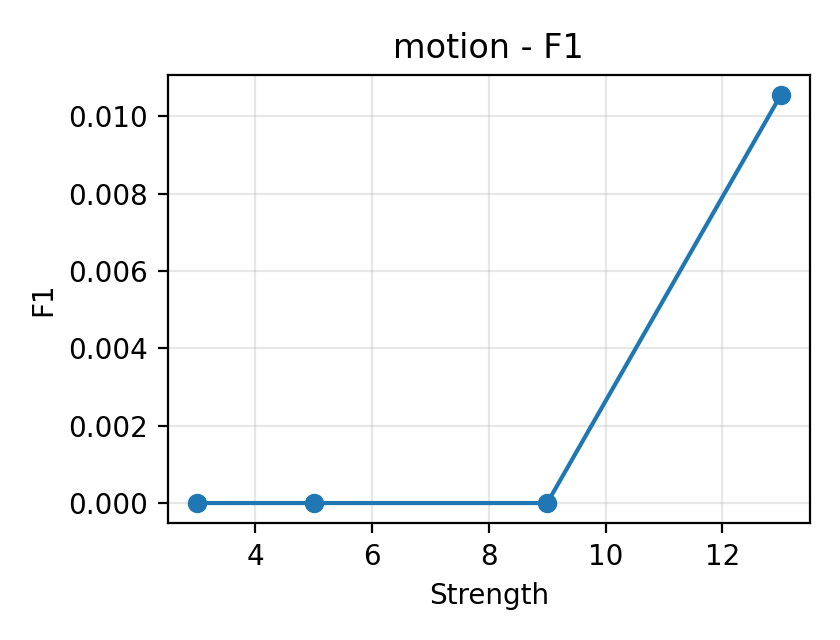
\includegraphics[width=0.9\textwidth]{outputs_stage5_robustness_motion_f1.png}
    \caption*{Motion Blur vs F1}
\end{figure}
\end{column}
\end{columns}
\end{frame}

% ============================================
% Slide 16: APP Interface Demo
% ============================================
\begin{frame}{APP Interface Demo}
\begin{columns}[T]
\begin{column}{0.5\textwidth}
\textbf{Simple 3-Step Workflow}
\begin{enumerate}
    \item Import video/image (local, no cloud upload)
    \item Local detection
    \item Output result
\end{enumerate}

\vspace{0.5em}
\textbf{Features}
\begin{itemize}
    \item Overall probability + keyframe heatmap
    \item Two-stage results display
    \item Stage 1 quick scan, Stage 2 refinement
    \item Average latency: $\sim$180ms
\end{itemize}
\end{column}

\begin{column}{0.5\textwidth}
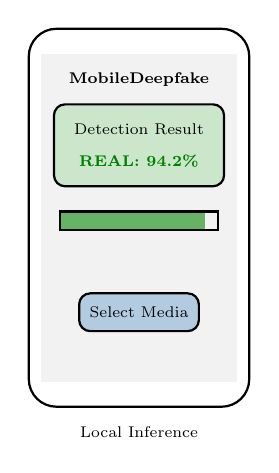
\begin{tikzpicture}[scale=0.8, transform shape]
    % Phone frame
    \draw[thick, rounded corners=10pt] (0,0) rectangle (3.5,6);

    % Screen
    \fill[gray!10] (0.2,0.4) rectangle (3.3,5.6);

    % UI elements
    \node[font=\scriptsize\bfseries] at (1.75,5.2) {MobileDeepfake};

    % Result box
    \draw[thick, fill=successgreen!20, rounded corners] (0.4,3.5) rectangle (3.1,4.8);
    \node[font=\scriptsize] at (1.75,4.4) {Detection Result};
    \node[font=\scriptsize\bfseries, successgreen] at (1.75,3.9) {REAL: 94.2\%};

    % Confidence bar
    \fill[successgreen!60] (0.5,2.8) rectangle (2.8,3.1);
    \draw[thick] (0.5,2.8) rectangle (3.0,3.1);

    % Import button
    \draw[thick, fill=primaryblue!30, rounded corners] (0.8,1.2) rectangle (2.7,1.8);
    \node[font=\scriptsize] at (1.75,1.5) {Select Media};

    % Label
    \node[below, font=\scriptsize] at (1.75,-0.2) {Local Inference};
\end{tikzpicture}
\end{column}
\end{columns}
\end{frame}

% ============================================
% Slide 17: Engineering Implementation
% ============================================
\begin{frame}{Engineering Implementation}
\begin{columns}[T]
\begin{column}{0.5\textwidth}
\textbf{Model Architecture}
\begin{center}
\scriptsize
\begin{tabular}{llcc}
\toprule
\textbf{Stage} & \textbf{Model} & \textbf{FP32 TS} & \textbf{FP32 ONNX} \\
\midrule
Stage 1 & MobileNetV4 & 37.3 MB & $\sim$37.5 MB \\
Stage 2 & EfficientNetV2-B3 & 49.6 MB & $\sim$52 MB \\
\bottomrule
\end{tabular}
\end{center}

\vspace{0.5em}
\textbf{Optimization \& Deployment}
\begin{itemize}
    \item INT8 post-training quantization
    \item ONNX export for cross-platform
    \item ONNX Runtime Android 1.19.0
    \item Multi-thread pipeline (4 threads)
\end{itemize}
\end{column}

\begin{column}{0.5\textwidth}
\textbf{Engineering Highlights}
\begin{itemize}
    \item End-to-end reproducible
    \item Semi-automated export pipeline
    \item Face detection on-device
    \item CPU baseline (GPU/NNAPI as future work)
\end{itemize}

\vspace{0.5em}
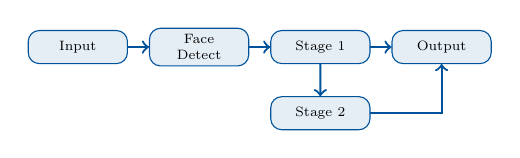
\begin{tikzpicture}[scale=0.7, transform shape,
    box/.style={rectangle, draw=primaryblue, fill=primaryblue!10,
                minimum width=1.8cm, minimum height=0.6cm, align=center,
                rounded corners, font=\scriptsize},
    arrow/.style={->, thick, primaryblue}]

\node[box] (in) at (0,0) {Input};
\node[box] (det) at (2.2,0) {Face\\Detect};
\node[box] (s1) at (4.4,0) {Stage 1};
\node[box] (s2) at (4.4,-1.2) {Stage 2};
\node[box] (out) at (6.6,0) {Output};

\draw[arrow] (in) -- (det);
\draw[arrow] (det) -- (s1);
\draw[arrow] (s1) -- (out);
\draw[arrow] (s1) -- (s2);
\draw[arrow] (s2) -| (out);
\end{tikzpicture}
\end{column}
\end{columns}
\end{frame}

% ============================================
% Slide 17.5: PC vs Mobile Deployment Comparison
% ============================================
\begin{frame}{PC vs Mobile Deployment Comparison}
\begin{columns}[T]
\begin{column}{0.55\textwidth}
\textbf{Performance Comparison}
\begin{center}
\scriptsize
\begin{tabular}{lrr}
\toprule
\textbf{Metric} & \textbf{PC} & \textbf{Mobile} \\
\midrule
Accuracy & 96.5\% & 92.8\% \\
FNR & 0.6\% & 2.5\% \\
FPR & 3.5\% & 12.5\% \\
Stage2 Rate & 1.2\% & 7.2\% \\
\midrule
Latency & -- & $\sim$180 ms \\
\bottomrule
\end{tabular}
\end{center}

\vspace{0.3em}
\textbf{Model Size Comparison}
\begin{center}
\scriptsize
\begin{tabular}{lrrr}
\toprule
\textbf{Stage} & \textbf{FP32 TS} & \textbf{INT8 TS} & \textbf{FP32 ONNX} \\
\midrule
Stage 1 & 37.3 MB & \highlight{10.1 MB} & 37.5 MB \\
Stage 2 & 49.6 MB & \highlight{13.4 MB} & 52 MB \\
\bottomrule
\end{tabular}
\end{center}

{\scriptsize \textit{Android deployment uses FP32 ONNX; INT8 available for size-constrained scenarios.}}
\end{column}

\begin{column}{0.45\textwidth}
\textbf{Latency Breakdown (Xiaomi 13)}
\begin{center}
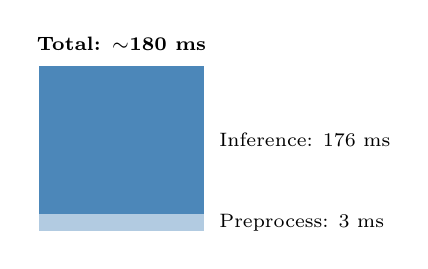
\begin{tikzpicture}[scale=0.7]
    % Stacked bar
    \fill[primaryblue!30] (0,0) rectangle (3,0.3);
    \fill[primaryblue!70] (0,0.3) rectangle (3,3);

    % Labels
    \node[right, font=\scriptsize] at (3.1,0.15) {Preprocess: 3 ms};
    \node[right, font=\scriptsize] at (3.1,1.65) {Inference: 176 ms};

    % Total
    \node[above, font=\scriptsize\bfseries] at (1.5,3.1) {Total: $\sim$180 ms};
\end{tikzpicture}
\end{center}

\vspace{0.3em}
\textbf{Calibration Parameters}
\begin{itemize}
\setlength\itemsep{0.1em}
    \item Temperature: T $\approx$ 1.34
    \item ECE reduced by \highlight{79\%}
    \item Thresholds: $\tau_{low}$=0.05, $\tau_{high}$=0.55
    \item 4\% accuracy for on-device privacy and latency
\end{itemize}
\end{column}
\end{columns}
\end{frame}

% ============================================
% Slide 18: Work Summary
% ============================================
\begin{frame}{Work Summary}
\begin{columns}[T]
\begin{column}{0.55\textwidth}
\textbf{Four Major Contributions}

\begin{enumerate}
    \item \highlight{Two-Stage Cascade Detection}
    \begin{itemize}
        \item FNR $\approx$ 0.6\%, Escalation $\approx$ 1.2\%
    \end{itemize}

    \item \highlight{Multi-Dataset Training \& Evaluation}
    \begin{itemize}
        \item Revealed distribution shift challenge
    \end{itemize}

    \item \highlight{End-to-End 6-Stage Pipeline}
    \begin{itemize}
        \item Preprocessing to mobile export
    \end{itemize}

    \item \highlight{Mobile Deployment}
    \begin{itemize}
        \item 92.8\% accuracy, $\sim$180ms latency
    \end{itemize}
\end{enumerate}
\end{column}

\begin{column}{0.45\textwidth}
\begin{block}{Key Metrics}
\begin{center}
\scriptsize
\begin{tabular}{llr}
\toprule
\textbf{Scenario} & \textbf{Metric} & \textbf{Value} \\
\midrule
PC In-domain & FNR & $\sim$0.6\% \\
PC In-domain & Stage2 Rate & $\sim$1.2\% \\
\midrule
Mobile (Xiaomi 13) & Accuracy & \highlight{92.8\%} \\
Mobile (Xiaomi 13) & Latency & $\sim$180ms \\
\midrule
OOD (Eval-2024) & F1 & $<$0.30 \\
\bottomrule
\end{tabular}
\end{center}
\end{block}

\vspace{0.5em}
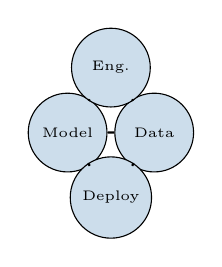
\begin{tikzpicture}[scale=0.55]
    \node[draw, circle, fill=primaryblue!20, minimum size=1cm, font=\tiny] (m) at (0,0) {Model};
    \node[draw, circle, fill=primaryblue!20, minimum size=1cm, font=\tiny] (d) at (2,0) {Data};
    \node[draw, circle, fill=primaryblue!20, minimum size=1cm, font=\tiny] (e) at (1,1.5) {Eng.};
    \node[draw, circle, fill=primaryblue!20, minimum size=1cm, font=\tiny] (dep) at (1,-1.5) {Deploy};

    \draw[thick] (m) -- (d) -- (e) -- (m) -- (dep) -- (d);
\end{tikzpicture}
\end{column}
\end{columns}
\end{frame}

% ============================================
% Slide 19: Limitations and Future Work
% ============================================
\begin{frame}{Limitations and Future Work}
\begin{columns}[T]
\begin{column}{0.5\textwidth}
\textbf{Current Limitations}
\begin{center}
\scriptsize
\begin{tabular}{lp{4cm}}
\toprule
\textbf{Limitation} & \textbf{Description} \\
\midrule
Distribution Shift & Cross-dataset F1$<$0.30 \\
Adversarial Attack & Not systematically evaluated \\
Device Coverage & Only Xiaomi 13 tested \\
Temporal Modeling & Frame-level, no video fusion \\
\bottomrule
\end{tabular}
\end{center}
\end{column}

\begin{column}{0.5\textwidth}
\textbf{Future Directions}
\begin{itemize}
    \item \highlight{Domain Adaptation/Generalization}
    \begin{itemize}
        \item Mitigate distribution shift
    \end{itemize}
    \item \highlight{Temporal Modeling}
    \begin{itemize}
        \item RNN/Transformer for video-level
    \end{itemize}
    \item \highlight{Adversarial Defense}
    \begin{itemize}
        \item Adversarial training
    \end{itemize}
    \item \highlight{Multi-Platform}
    \begin{itemize}
        \item More SoCs, iOS support
    \end{itemize}
\end{itemize}
\end{column}
\end{columns}

\vspace{0.5em}
\begin{center}
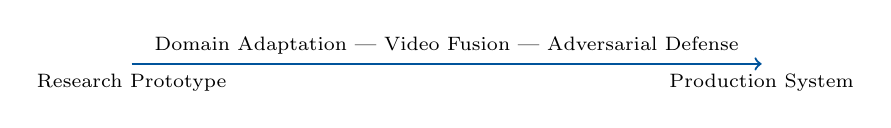
\begin{tikzpicture}
    \draw[->, thick, primaryblue] (0,0) -- (8,0);
    \node[below] at (0,0) {\scriptsize Research Prototype};
    \node[below] at (8,0) {\scriptsize Production System};
    \node[above, font=\scriptsize] at (4,0) {Domain Adaptation | Video Fusion | Adversarial Defense};
\end{tikzpicture}
\end{center}
\end{frame}

% ============================================
% Slide 20: Acknowledgments and Q&A
% ============================================
\begin{frame}
\begin{center}
\vspace{2em}
{\Huge Thank You!}

\vspace{2em}
{\large Questions \& Discussion}

\end{center}
\end{frame}

% ============================================
% Backup Slides (if needed)
% ============================================
\appendix

\begin{frame}{Backup: Stage1 Calibration}
\begin{center}
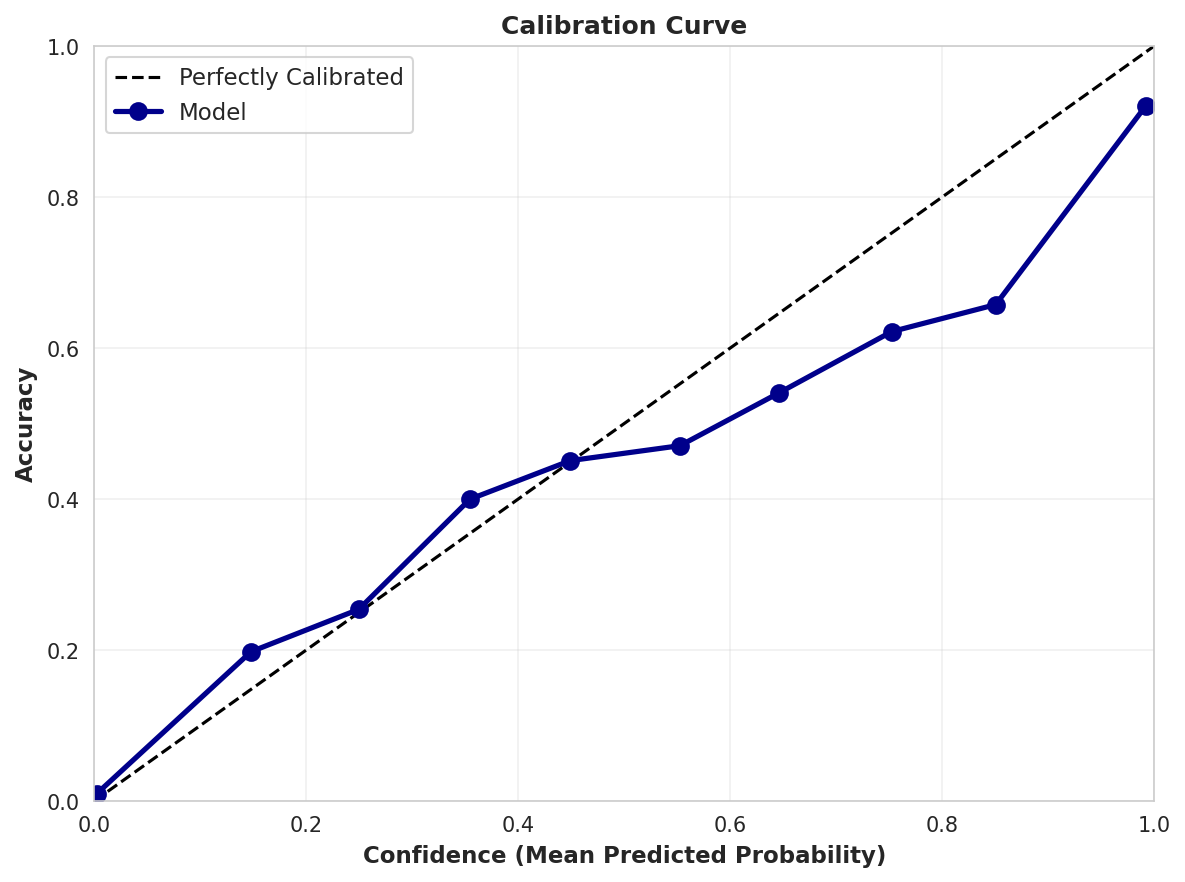
\includegraphics[width=0.6\textwidth]{outputs_stage1_run_20251023_034316_03_calibration.png}
\end{center}
\end{frame}

\begin{frame}{Backup: Stage1 Confusion Matrix}
\begin{center}
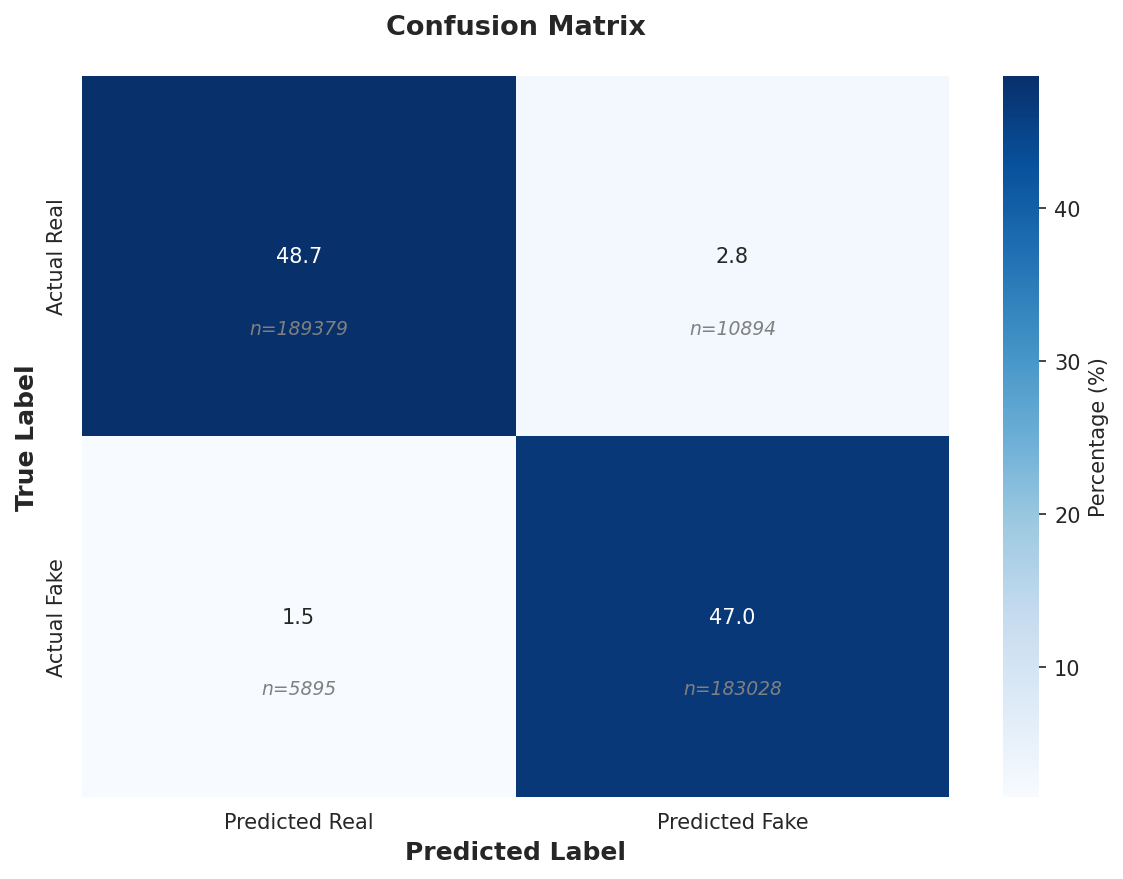
\includegraphics[width=0.5\textwidth]{outputs_stage1_run_20251023_034316_confusion_matrix.png}
\end{center}
\end{frame}

\begin{frame}{Backup: FNR Heatmap}
\begin{center}
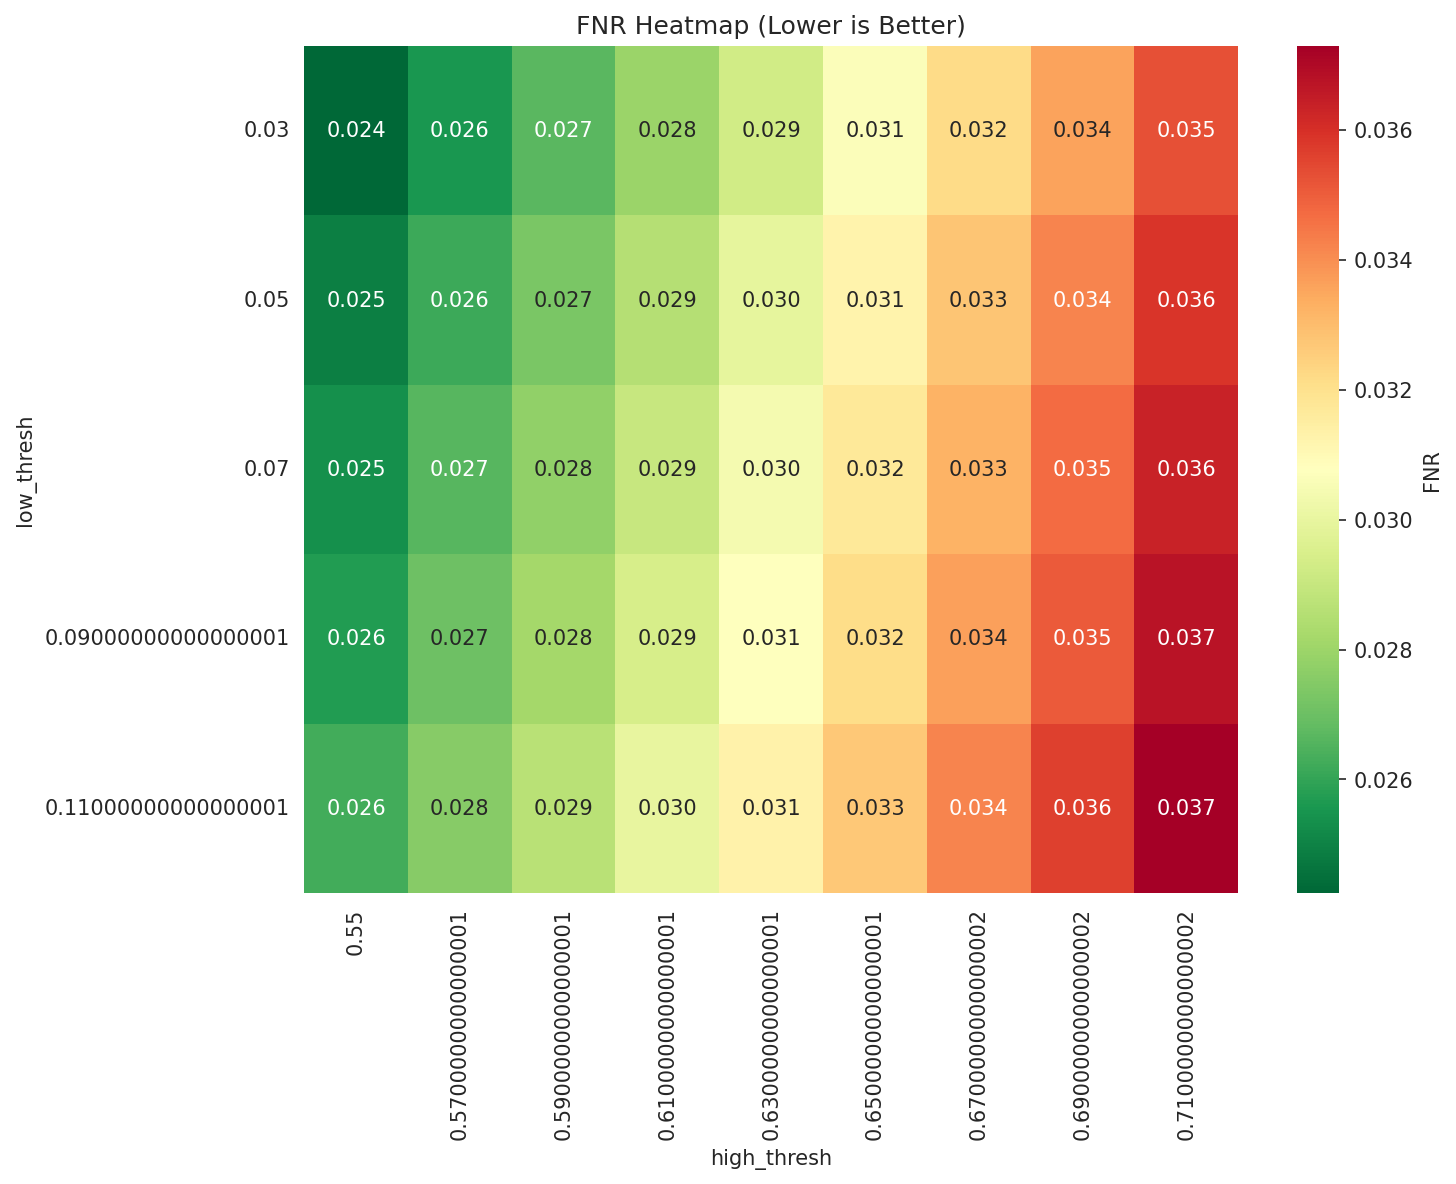
\includegraphics[width=0.7\textwidth]{outputs_stage4_run_20251031_075851_heatmap_fnr.png}
\end{center}
\end{frame}

\begin{frame}{Backup: Gaussian Noise Robustness}
\begin{center}
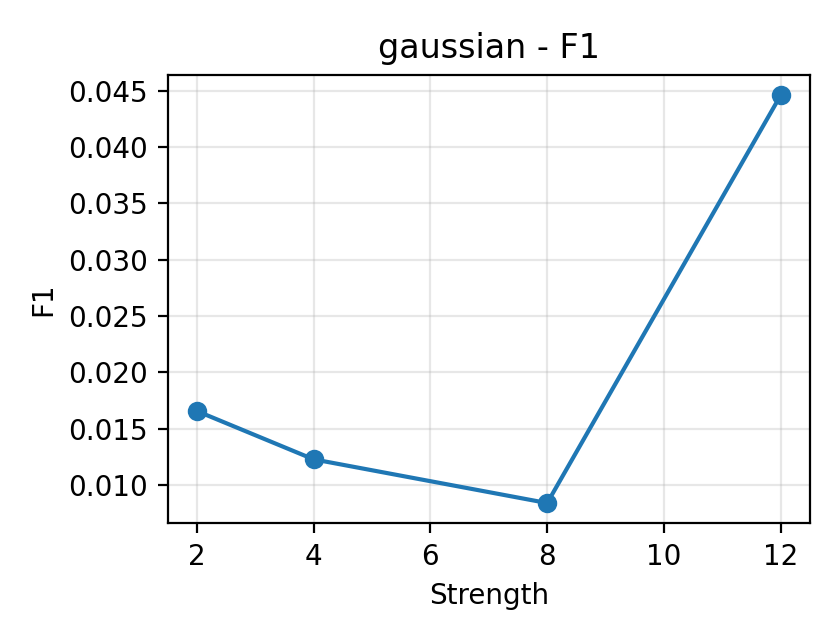
\includegraphics[width=0.7\textwidth]{outputs_stage5_robustness_gaussian_f1.png}
\end{center}
\end{frame}

\end{document}
